\documentclass{article}%
\usepackage[T1]{fontenc}%
\usepackage[utf8]{inputenc}%
\usepackage{lmodern}%
\usepackage{textcomp}%
\usepackage{lastpage}%
\usepackage{parskip}%
\usepackage[top=1.2in,bottom=1in,left=0.6in,right=0.6in,headsep=0.8in]{geometry}%
\usepackage{amsmath}%
\usepackage{graphicx}%
\usepackage{needspace}%
\usepackage{color}%
\usepackage{longtable}%
\usepackage{multirow}%
\usepackage[table]{xcolor}%
\usepackage{fancyhdr}%
\usepackage{tabularx}%
%
\definecolor{OsdagGreen}{HTML}{D5DF93}%
\fancypagestyle{header}{ 
\renewcommand{\headrulewidth}{0pt}%
\renewcommand{\footrulewidth}{0pt}%
\fancyhead{ 
}%
\fancyfoot{ 
}%
\fancyhead[C]{ 
\begin{tabularx}{\textwidth}{|l|p{6cm}|l|X|}%
\hline%
\rowcolor{OsdagGreen}%
Company Name&&Project Title&\\%
\hline%
\rowcolor{OsdagGreen}%
Group/Team Name&&Subtitle&\\%
\hline%
\rowcolor{OsdagGreen}%
Designer&&Job Number&\\%
\hline%
\rowcolor{OsdagGreen}%
Date&30 /04 /2020&Client&\\%
\hline%
\end{tabularx}
}%
\fancyfoot[R]{ 
Page \thepage\ of \pageref{LastPage}
}
}%
%
\begin{document}%
\normalsize%
\pagestyle{header}%
\section{Input Parameters}%
\label{sec:InputParameters}%
\renewcommand{\arraystretch}{1.2}%
\begin{longtable}{|p{5cm}|p{2cm}|p{2cm}|p{2cm}|p{5cm}|}%
\hline%
\hline%
\multicolumn{3}{|c|}{Module}&\multicolumn{2}{|c|}{Beam Coverplate Connection}\\%
\hline%
\hline%
\multicolumn{3}{|c|}{MainModule}&\multicolumn{2}{|c|}{Moment Connection}\\%
\hline%
\hline%
\multicolumn{3}{|c|}{Moment(kNm)*}&\multicolumn{2}{|c|}{10.0}\\%
\hline%
\hline%
\multicolumn{3}{|c|}{Shear(kN)*}&\multicolumn{2}{|c|}{10.0}\\%
\hline%
\hline%
\multicolumn{3}{|c|}{Axial (kN) *}&\multicolumn{2}{|c|}{10.0}\\%
\hline%
\hline%
\multicolumn{5}{|c|}{\textbf{Section}}\\%
\hline%
\hline%
\multirow{13}{*}{\includegraphics[width=5cm,height=5cm]{"E:/office _anjali/columnspliceanjali/Osdag3/ResourceFiles/images/ISection".png}}&\multicolumn{2}{|c|}{Beam Section *}&\multicolumn{2}{|c|}{UB 457 x 152 x 60}\\%
\cline{2%
-%
5}%
&\multicolumn{2}{|c|}{Preferences}&\multicolumn{2}{|c|}{Outside + Inside}\\%
\cline{2%
-%
5}%
&\multicolumn{2}{|c|}{Material *}&\multicolumn{2}{|c|}{E 250 (Fe 410 W)A}\\%
\cline{2%
-%
5}%
&\multicolumn{2}{|c|}{Ultimate strength, fu (MPa)}&\multicolumn{2}{|c|}{410}\\%
\cline{2%
-%
5}%
&Yield Strength , fy (MPa)&230&R2(mm)&0.0\\%
\cline{2%
-%
5}%
&Mass&59.8&Iz(mm4)&255000000.0\\%
\cline{2%
-%
5}%
&Area(mm2) {-} A&7620.0&Iy(mm4)&7940000.0\\%
\cline{2%
-%
5}%
&D(mm)&455.0&rz(mm)&183.0\\%
\cline{2%
-%
5}%
&B(mm)&152.9&ry(mm)&32.0\\%
\cline{2%
-%
5}%
&t(mm)&8.1&Zz(mm3)&1122000.0\\%
\cline{2%
-%
5}%
&T(mm)&13.3&Zy(mm3)&104000.0\\%
\cline{2%
-%
5}%
&FlangeSlope&90&Zpz(mm3)&1287000.0\\%
\cline{2%
-%
5}%
&R1(mm)&10.2&Zpy(mm3)&104000.0\\%
\cline{2%
-%
5}%
\hline%
\multicolumn{5}{|c|}{\textbf{Bolt Details}}\\%
\hline%
\hline%
\multicolumn{3}{|c|}{Diameter(mm)*}&\multicolumn{2}{|c|}{{[}12.0, 16.0, 20.0, 24.0, 30.0, 36.0{]}}\\%
\hline%
\hline%
\multicolumn{3}{|c|}{Grade *}&\multicolumn{2}{|c|}{{[}3.6, 4.6, 4.8, 5.6, 5.8, 6.8, 8.8, 9.8, 10.9, 12.9{]}}\\%
\hline%
\hline%
\multicolumn{3}{|c|}{Type *}&\multicolumn{2}{|c|}{Bearing Bolt}\\%
\hline%
\hline%
\multicolumn{3}{|c|}{Bolt.fu}&\multicolumn{2}{|c|}{600.0}\\%
\hline%
\hline%
\multicolumn{3}{|c|}{Bolt.fy}&\multicolumn{2}{|c|}{479.9999999999999}\\%
\hline%
\hline%
\multicolumn{3}{|c|}{Bolt hole type}&\multicolumn{2}{|c|}{Standard}\\%
\hline%
\hline%
\multicolumn{3}{|c|}{Slip factor (µ\_f)}&\multicolumn{2}{|c|}{0.3}\\%
\hline%
\hline%
\multicolumn{3}{|c|}{Type of edges}&\multicolumn{2}{|c|}{a {-} Sheared or hand flame cut}\\%
\hline%
\hline%
\multicolumn{3}{|c|}{Gap between beam and <br>support (mm)}&\multicolumn{2}{|c|}{10.0}\\%
\hline%
\hline%
\multicolumn{3}{|c|}{Are the members exposed to <br>corrosive influences}&\multicolumn{2}{|c|}{False}\\%
\hline%
\end{longtable}

%
\Needspace{10\baselineskip}%
\section{Design Checks}%
\label{sec:DesignChecks}%
\subsection{Member Capacity}%
\label{subsec:MemberCapacity}%
\renewcommand{\arraystretch}{1.2}%
\begin{longtable}{|p{4cm}|p{5cm}|p{5.5cm}|p{1.5cm}|}%
\hline%
\rowcolor{OsdagGreen}%
Check&Required&Provided&Remarks\\%
\hline%
\endhead%
\hline%
Axial Capacity Member Ac (kN)&&$\begin{aligned} Ac &=\frac{A*f_y}{\gamma_{m0} *1000}\\ &=\frac{7620.0*230}{1.1* 1000}\\ &=1593.27\end{aligned}$&\\%
\hline%
Shear Capacity Member Sc (kN)&&$\begin{aligned} S_c &= \frac{A_v*f_y}{\sqrt{3}*\gamma_{mo} *1000}\\ &=\frac{428.4*8.1*230}{\sqrt{3}*1.1 *1000}\\ &=418.89869\end{aligned}$&\\%
\hline%
Plastic Moment Capacity Pmc (kNm)&&$\begin{aligned} Pmc &= \frac{\beta_b * Z_p *fy}{\gamma_{mo} * 1000000}\\ &=\frac{1*371641*230}{1.1 * 1000000}\\ &=77.71\end{aligned}$&\\%
\hline%
Moment Deformation Criteria Mdc (kNm)&&$\begin{aligned} Mdc &= \frac{1.5 *Z_e *fy}{1.1}\\ &= \frac{1.5 *1122000.0*230}{1.1}\\ &= 351.9\end{aligned}$&\\%
\hline%
Moment Capacity Member Mc (kNm)&&$\begin{aligned} M_c &= min(Pmc,Mdc)\\ &=min(77.71,351.9)\\ &=77.71\end{aligned}$&\\%
\hline%
\end{longtable}

%
\subsection{Load Considered}%
\label{subsec:LoadConsidered}%
\renewcommand{\arraystretch}{1.2}%
\begin{longtable}{|p{4cm}|p{5cm}|p{5.5cm}|p{1.5cm}|}%
\hline%
\rowcolor{OsdagGreen}%
Check&Required&Provided&Remarks\\%
\hline%
\endhead%
\hline%
Applied Axial Load Au (kN)&$\begin{aligned} Ac_{min} &= 0.3 * A_c\\ &= 0.3 *1593.27\\ &=477.98\end{aligned}$&$\begin{aligned} Au &= max(A,Ac_{min} )\\ &= max( 10.0,477.98)\\ &=477.98\end{aligned}$&Pass\\%
\hline%
Applied Shear Load Vu (kN)&$\begin{aligned} Sc_{min} &= 0.6 * A_c\\ &= 0.6 *418.9\\ &=251.34\end{aligned}$&$\begin{aligned} Vu &= max(V,Vc_{min})\\ &=  max(10.0,251.34)\\ &=251.34\end{aligned}$&Pass\\%
\hline%
Applied Moment Load Mu (kNm)&$\begin{aligned} Mc_{min} &= 0.5 * M_c\\ &= 0.5 *77.71\\ &=38.85\end{aligned}$&$\begin{aligned} Mu &= max(M,Mc_{min} )\\ &= max(10.0,38.85)\\ &=38.85\end{aligned}$&Pass\\%
\hline%
Forces Carried by Web&&$\begin{aligned}A_w &= Axial~ force~ in~ web  \\   &= \frac{(D- 2*T)*t* Au }{A} \\ &= \frac{(455.0- 2*13.3)*8.1*477.98 }{7620.0} \\ &=217.67\\ M_w &= Moment ~in ~web  \\  &= \frac{Z_w * Mu}{Z} \\ &= \frac{371641 * 38.85}{1287000.0} \\ &=11.22\end{aligned}$&\\%
\hline%
Forces Carried by Flange&&$\begin{aligned} A_f&= Axial~force~ in ~flange  \\ &= \frac{Au * B *T}{A} \\ &= \frac{477.98 * 152.9*13.3}{7620.0} \\ &=127.56\\ M_f& =Moment~ in~ flange \\  & = Mu-M_w\\ &= 38.85-11.22\\ &=27.63\\  f_f& =flange~force  \\ & = \frac{M_f *1000}{D-T} + A_f \\ &= \frac{27.63}{455.0-13.3} +127.56 \\ &=190.12\end{aligned}$&\\%
\hline%
\end{longtable}

%
\subsection{Flange Bolt Checks}%
\label{subsec:FlangeBoltChecks}%
\renewcommand{\arraystretch}{1.2}%
\begin{longtable}{|p{4cm}|p{5cm}|p{5.5cm}|p{1.5cm}|}%
\hline%
\rowcolor{OsdagGreen}%
Check&Required&Provided&Remarks\\%
\hline%
\endhead%
\hline%
Shear Capacity (kN)&&$\begin{aligned}V_{dsb} &= \frac{f_ub ~n_n~ A_{nb}}{\sqrt{3} ~\gamma_{mb}}\\ &= \frac{600.0*2*84.3}{\sqrt{3}~*~1.25}\\ &= 46.72\end{aligned}$&\\%
\hline%
Bearing Capacity (kN)&&$\begin{aligned}V_{dpb} &= \frac{2.5~ k_b~ d~ t~ f_u}{\gamma_{mb}}\\ &= \frac{2.5~*0.52*12.0*13.3*410}{1.25}\\ &=67.95\end{aligned}$&\\%
\hline%
Bolt Capacity (kN)&&$\begin{aligned}V_{db} &= min~ (V_{dsb}, V_{dpb})\\ &= min~ (46.72,67.95)\\ &=46.72\end{aligned}$&\\%
\hline%
No of Bolts&$\begin{aligned}R_{u} &= \sqrt{V_u^2+A_u^2}\\ n_{trial} &= R_u/ V_{bolt}\\ R_{u} &= \frac{\sqrt{0.0^2+190.12^2}}{46.72}\\ &=10\end{aligned}$&12&\\%
\hline%
No of Columns&&6&\\%
\hline%
No of Rows&&2&\\%
\hline%
Min. Pitch (mm)&$\begin{aligned}p/g_{min}&= 2.5 ~ d&\\ =&2.5*12.0&=30.0\end{aligned}$&30&Pass\\%
\hline%
Max. Pitch (mm)&$\begin{aligned}p/g_{max} &=\min(32~t,~300~mm)&\\ &=\min(32 *~8.0,~ 300 ~mm)\\&=300\end{aligned}$&30&Pass\\%
\hline%
Min. Gauge (mm)&$\begin{aligned}p/g_{min}&= 2.5 ~ d&\\ =&2.5*12.0&=30.0\end{aligned}$&0.0&N/A\\%
\hline%
Max. Gauge (mm)&$\begin{aligned}p/g_{max} &=\min(32~t,~300~mm)&\\ &=\min(32 *~8.0,~ 300 ~mm)\\&=300\end{aligned}$&0.0&N/A\\%
\hline%
Min. End Distance (mm)&$\begin{aligned}e/e`_{min} &=[1.5~or~ 1.7] * d_0\\ &=1.7*13.0=22.1 \end{aligned}$&25&Pass\\%
\hline%
Max. End Distance (mm)&$\begin{aligned}e/e`_{max} &= 12~ t~ \varepsilon&\\ \varepsilon &= \sqrt{\frac{250}{f_y}}\\ e/e`_{max}&=12 ~*8.0*\sqrt{\frac{250}{230}}\\ &=99.84\\ \end{aligned}$&25&Pass\\%
\hline%
Min. Edge Distance (mm)&$\begin{aligned}e/e`_{min} &=[1.5~or~ 1.7] * d_0\\ &=1.7*13.0=22.1 \end{aligned}$&31.1&Pass\\%
\hline%
Max. Edge Distance (mm)&$\begin{aligned}e/e`_{max} &= 12~ t~ \varepsilon&\\ \varepsilon &= \sqrt{\frac{250}{f_y}}\\ e/e`_{max}&=12 ~*8.0*\sqrt{\frac{250}{230}}\\ &=99.84\\ \end{aligned}$&31.1&Pass\\%
\hline%
\end{longtable}

%
\subsection{Web Bolt Checks}%
\label{subsec:WebBoltChecks}%
\renewcommand{\arraystretch}{1.2}%
\begin{longtable}{|p{4cm}|p{6cm}|p{5.5cm}|p{1.5cm}|}%
\hline%
\rowcolor{OsdagGreen}%
Check&Required&Provided&Remarks\\%
\hline%
\endhead%
\hline%
Shear Capacity (kN)&&$\begin{aligned}V_{dsb} &= \frac{f_ub ~n_n~ A_{nb}}{\sqrt{3} ~\gamma_{mb}}\\ &= \frac{600.0*2*84.3}{\sqrt{3}~*~1.25}\\ &= 46.72\end{aligned}$&\\%
\hline%
Bearing Capacity (kN)&&$\begin{aligned}V_{dpb} &= \frac{2.5~ k_b~ d~ t~ f_u}{\gamma_{mb}}\\ &= \frac{2.5~*0.52*12.0*8.1*410}{1.25}\\ &=41.38\end{aligned}$&\\%
\hline%
Bolt Capacity (kN)&&$\begin{aligned}V_{db} &= min~ (V_{dsb}, V_{dpb})\\ &= min~ (46.72,41.38)\\ &=41.38\end{aligned}$&\\%
\hline%
No of Bolts&$\begin{aligned}R_{u} &= \sqrt{V_u^2+A_u^2}\\ n_{trial} &= R_u/ V_{bolt}\\ R_{u} &= \frac{\sqrt{251.34^2+217.67^2}}{41.38}\\ &=18\end{aligned}$&32&\\%
\hline%
No of Columns&&4&\\%
\hline%
No of Rows&&8&\\%
\hline%
Min. Pitch (mm)&$\begin{aligned}p/g_{min}&= 2.5 ~ d&\\ =&2.5*12.0&=30.0\end{aligned}$&30&Pass\\%
\hline%
Max. Pitch (mm)&$\begin{aligned}p/g_{max} &=\min(32~t,~300~mm)&\\ &=\min(32 *~6.0,~ 300 ~mm)\\&=300\end{aligned}$&30&Pass\\%
\hline%
Min. Gauge (mm)&$\begin{aligned}p/g_{min}&= 2.5 ~ d&\\ =&2.5*12.0&=30.0\end{aligned}$&45&Pass\\%
\hline%
Max. Gauge (mm)&$\begin{aligned}p/g_{max} &=\min(32~t,~300~mm)&\\ &=\min(32 *~6.0,~ 300 ~mm)\\&=300\end{aligned}$&45&Pass\\%
\hline%
Min. End Distance (mm)&$\begin{aligned}e/e`_{min} &=[1.5~or~ 1.7] * d_0\\ &=1.7*13.0=22.1 \end{aligned}$&25&Pass\\%
\hline%
Max. End Distance (mm)&$\begin{aligned}e/e`_{max} &= 12~ t~ \varepsilon&\\ \varepsilon &= \sqrt{\frac{250}{f_y}}\\ e/e`_{max}&=12 ~*6.0*\sqrt{\frac{250}{230}}\\ &=74.88\\ \end{aligned}$&25&Pass\\%
\hline%
Min. Edge Distance (mm)&$\begin{aligned}e/e`_{min} &=[1.5~or~ 1.7] * d_0\\ &=1.7*13.0=22.1 \end{aligned}$&25&Pass\\%
\hline%
Max. Edge Distance (mm)&$\begin{aligned}e/e`_{max} &= 12~ t~ \varepsilon&\\ \varepsilon &= \sqrt{\frac{250}{f_y}}\\ e/e`_{max}&=12 ~*6.0*\sqrt{\frac{250}{230}}\\ &=74.88\\ \end{aligned}$&25&Pass\\%
\hline%
\end{longtable}

%
\subsection{Inner and Outer flange plate Checks}%
\label{subsec:InnerandOuterflangeplateChecks}%
\renewcommand{\arraystretch}{1.2}%
\begin{longtable}{|p{4cm}|p{6cm}|p{5.5cm}|p{1.5cm}|}%
\hline%
\rowcolor{OsdagGreen}%
Check&Required&Provided&Remarks\\%
\hline%
\endhead%
\hline%
Min. Plate Height (mm)&$\begin{aligned}min~flange~plate~ht &= beam~width\\ &=152.9\end{aligned}$&152.9&Pass\\%
\hline%
Min. Plate Length (mm)&$\begin{aligned} & 2[2*e_{min} + ({\frac{bolt~lines}{2}}-1) * p_{min})]\\ & +\frac{gap}{2}]\\ &=2*[(2*22.1 + (\frac{6}{2}-1) * 30.0\\ &= + \frac{10.0}{2}]\\ &=218.4\end{aligned}$&230.0&Pass\\%
\hline%
Min. Inner Plate Height (mm)&$\begin{aligned}&= \frac{B -t- (2*R1)}{2}\\ &=\frac{152.9 -8.1 - 2*10.2}{2}\\ &=62.2\end{aligned}$&62.2&Pass\\%
\hline%
Max. Inner Plate Height (mm)&$\begin{aligned}&= \frac{B -t- (2*R1)}{2}\\ &=\frac{152.9 -8.1 - 2*10.2}{2}\\ &=62.2\end{aligned}$&62.2&Pass\\%
\hline%
Min. Inner Plate Length (mm)&$\begin{aligned} & 2[2*e_{min} + ({\frac{bolt~lines}{2}}-1) * p_{min})]\\ & +\frac{gap}{2}]\\ &=2*[(2*22.1 + (\frac{6}{2}-1) * 30.0\\ &= + \frac{10.0}{2}]\\ &=218.4\end{aligned}$&230.0&Pass\\%
\hline%
Min.Plate Thickness (mm)&$\begin{aligned} t_w=6.65\end{aligned}$&8.0&Pass\\%
\hline%
\end{longtable}

%
\subsection{Member Checks}%
\label{subsec:MemberChecks}%
\renewcommand{\arraystretch}{1.2}%
\begin{longtable}{|p{4cm}|p{6cm}|p{5.5cm}|p{1.5cm}|}%
\hline%
\rowcolor{OsdagGreen}%
Check&Required&Provided&Remarks\\%
\hline%
\endhead%
\hline%
Flange Tension Yielding Capacity (kN)&&$\begin{aligned} T_{dg} &= \frac{l*t*f_y}{\gamma_{mo}}\\ &=\frac{152.9*13.3*230}{\sqrt{3}*1.1}\\ &=425.2\end{aligned}$&\\%
\hline%
Flange Tension Rupture Capacity (kN)&&$\begin{aligned} T_{dn} &= \frac{0.9*A_{n}*f_u}{\gamma_{m1}}\\ &=\frac{0.9*(152.9-2*13.0)*13.3*410}{1.25}\\ &=498.23\end{aligned}$&\\%
\hline%
Flange Block Shear Capacity (kN)&&$\begin{aligned}T_{db1} &= \frac{A_{vg} f_{y}}{\sqrt{3} \gamma_{m0}} + \frac{0.9 A_{tn} f_{u}}{\gamma_{m1}}\\ T_{db2} &= \frac{0.9*A_{vn} f_{u}}{\sqrt{3} \gamma_{m1}} + \frac{A_{tg} f_{y}}{\gamma_{m0}}\\ T_{db} &= min(T_{db1}, T_{db2})= 410983.346\end{aligned}$&\\%
\hline%
Flange Tension Capacity (kN)&190.12&$\begin{aligned} T_d &= Min(T_{dg},T_{dn},T_{db})\\ &= Min(425.2,498.23,410.98)\\ &=410.98\end{aligned}$&Pass\\%
\hline%
Web Tension Yielding Capacity (kN)&&$\begin{aligned} T_{dg} &= \frac{l*t*f_y}{\gamma_{mo}}\\ &=\frac{428.4*8.1*230}{\sqrt{3}*1.1}\\ &=725.55\end{aligned}$&\\%
\hline%
Web Tension Rupture Capacity (kN)&&$\begin{aligned} T_{dn} &= \frac{0.9*A_{n}*f_u}{\gamma_{m1}}\\ &=\frac{0.9*(428.4-8*13.0)*8.1*410}{1.25}\\ &=775.68\end{aligned}$&\\%
\hline%
Web Block Shear Capacity (kN)&&$\begin{aligned}T_{db1} &= \frac{A_{vg} f_{y}}{\sqrt{3} \gamma_{m0}} + \frac{0.9 A_{tn} f_{u}}{\gamma_{m1}}\\ T_{db2} &= \frac{0.9*A_{vn} f_{u}}{\sqrt{3} \gamma_{m1}} + \frac{A_{tg} f_{y}}{\gamma_{m0}}\\ T_{db} &= min(T_{db1}, T_{db2})= 702.95\end{aligned}$&\\%
\hline%
Tension Capacity (kN)&217.67&$\begin{aligned} T_d &= Min(T_{dg},T_{dn},T_{db})\\ &= Min(725.55,775.68,702.95)\\ &=702.95\end{aligned}$&Pass\\%
\hline%
\end{longtable}

%
\subsection{Flange Plate Capacity Checks in axial{-}Outside/Inside }%
\label{subsec:FlangePlateCapacityChecksinaxial{-}Outside/Inside}%
\renewcommand{\arraystretch}{1.2}%
\begin{longtable}{|p{4cm}|p{6cm}|p{5.5cm}|p{1.5cm}|}%
\hline%
\rowcolor{OsdagGreen}%
Check&Required&Provided&Remarks\\%
\hline%
\endhead%
\hline%
Tension Yielding Capacity (kN)&&$\begin{aligned} T_{dg} &= \frac{l*t*f_y}{\gamma_{mo}}\\ &=\frac{277.3*8.0*230}{\sqrt{3}*1.1}\\ &=463.85\end{aligned}$&\\%
\hline%
Tension Rupture Capacity(kN)&&$\begin{aligned} T_{dn} &= \frac{0.9*A_{n}*f_u}{\gamma_{m1}}\\ &=\frac{0.9*(277.3-2*13.0)*8.0*410}{1.25}\\ &=593.47\end{aligned}$&\\%
\hline%
Block Shear Capacity (KN)&&$\begin{aligned}T_{db1} &= \frac{A_{vg} f_{y}}{\sqrt{3} \gamma_{m0}} + \frac{0.9 A_{tn} f_{u}}{\gamma_{m1}}\\ T_{db2} &= \frac{0.9*A_{vn} f_{u}}{\sqrt{3} \gamma_{m1}} + \frac{A_{tg} f_{y}}{\gamma_{m0}}\\ T_{db} &= min(T_{db1}, T_{db2})= 542.09\end{aligned}$&\\%
\hline%
Plate Tension Capacity  (kN)&190.12&$\begin{aligned} T_d &= Min(T_{dg},T_{dn},T_{db})\\ &= Min(463.85,593.47,542.09)\\ &=463.85\end{aligned}$&Pass\\%
\hline%
\end{longtable}

%
\subsection{Web Plate Capacity Checks in Axial}%
\label{subsec:WebPlateCapacityChecksinAxial}%
\renewcommand{\arraystretch}{1.2}%
\begin{longtable}{|p{4cm}|p{6cm}|p{5.5cm}|p{1.5cm}|}%
\hline%
\rowcolor{OsdagGreen}%
Check&Required&Provided&Remarks\\%
\hline%
\endhead%
\hline%
Tension Yielding Capacity (kN)&&$\begin{aligned} T_{dg} &= \frac{l*t*f_y}{\gamma_{mo}}\\ &=\frac{365*6.0*230}{\sqrt{3}*1.1}\\ &=915.82\end{aligned}$&\\%
\hline%
Tension Rupture Capacity(kN)&&$\begin{aligned} T_{dn} &= \frac{0.9*A_{n}*f_u}{\gamma_{m1}}\\ &=\frac{0.9*(365-8*13.0)*6.0*410}{1.25}\\ &=924.57\end{aligned}$&\\%
\hline%
Block Shear Capacity (KN)&&$\begin{aligned}T_{db1} &= \frac{A_{vg} f_{y}}{\sqrt{3} \gamma_{m0}} + \frac{0.9 A_{tn} f_{u}}{\gamma_{m1}}\\ T_{db2} &= \frac{0.9*A_{vn} f_{u}}{\sqrt{3} \gamma_{m1}} + \frac{A_{tg} f_{y}}{\gamma_{m0}}\\ T_{db} &= min(T_{db1}, T_{db2})= 1041.41\end{aligned}$&\\%
\hline%
Plate Tension Capacity (kN)&217.67&$\begin{aligned} T_d &= Min(T_{dg},T_{dn},T_{db})\\ &= Min(915.82,924.57,1041.41)\\ &=915.82\end{aligned}$&Pass\\%
\hline%
\end{longtable}

%
\subsection{Web Plate Capacity Checks in Shear}%
\label{subsec:WebPlateCapacityChecksinShear}%
\renewcommand{\arraystretch}{1.2}%
\begin{longtable}{|p{4cm}|p{6cm}|p{5.5cm}|p{1.5cm}|}%
\hline%
\rowcolor{OsdagGreen}%
Check&Required&Provided&Remarks\\%
\hline%
\endhead%
\hline%
Shear yielding Capacity (V\_dy) (kN)&&$\begin{aligned} V_{dg} &= \frac{A_v*f_y}{\sqrt{3}*\gamma_{mo}}\\ &=\frac{365*6.0*230}{\sqrt{3}*1.1}\\ &=528.75\end{aligned}$&\\%
\hline%
Shear Rupture Capacity (V\_dn) (kN)&&$\begin{aligned} V_{dn} &= \frac{0.75*A_{vn}*f_u}{\sqrt{3}*\gamma_{mo}}\\ &=0.9*(365-(2.0*13.0))*6.0*410\\ &=533.8\end{aligned}$&\\%
\hline%
Block Shear Capacity in Shear (V\_db) (kN)&&$\begin{aligned}T_{db1} &= \frac{A_{vg} f_{y}}{\sqrt{3} \gamma_{m0}} + \frac{0.9 A_{tn} f_{u}}{\gamma_{m1}}\\ T_{db2} &= \frac{0.9*A_{vn} f_{u}}{\sqrt{3} \gamma_{m1}} + \frac{A_{tg} f_{y}}{\gamma_{m0}}\\ T_{db} &= min(T_{db1}, T_{db2})= 633.96\end{aligned}$&\\%
\hline%
Plate Shear Capacity (kN)&251.34&$\begin{aligned} V_d &= Min(V_{dy},V_{dn},V_{db})\\ &= Min(528.75,533.8,1041.41)\\ &=528.75\end{aligned}$&Pass\\%
\hline%
\end{longtable}

%
\Needspace{10\baselineskip}%
\newpage%
\section{3D View}%
\label{sec:3DView}%


\begin{figure}[h!]%
\centering%
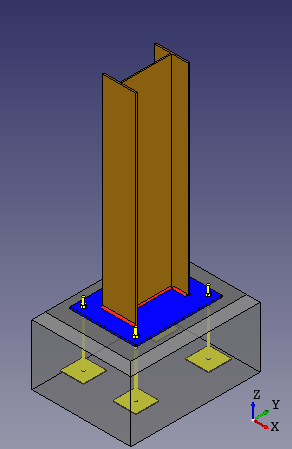
\includegraphics[width=\linewidth]{{"E:/office _anjali/columnspliceanjali/Osdag3./ResourceFiles/images/3d}.png}%
\caption{3D View}%
\end{figure}

%
\end{document}